\documentclass[11pt,twocolumn]{report}

\usepackage[margin=0.75in]{geometry}
\usepackage[T1]{fontenc}
\usepackage{amsmath}
\usepackage{amssymb}
\usepackage{bm}
\usepackage[strings]{underscore}
\usepackage{booktabs}
\usepackage{graphicx}
\usepackage{array}
\usepackage[round]{natbib}
\setcitestyle{aysep={}}          % (Author year), no comma
\usepackage{xcolor}
\usepackage{hyperref}
\hypersetup{colorlinks=true, linkcolor={red!50!black},
  citecolor={blue!50!black}, urlcolor={blue!80!black}}
\newcolumntype{L}[1]{>{\raggedright\arraybackslash}p{#1}}

% a caption sits above a table, and the class leaves no gap below it
\setlength{\belowcaptionskip}{8pt}
\setlength{\abovecaptionskip}{12pt}

\bibliographystyle{groundwater}

% shorthand used throughout the chapters
\newcommand{\mf}{MODFLOW~6}
\newcommand{\adj}{mf6adj}

\title{Supplemental Technical Information for \adj}
\author{}
\date{\today}

\begin{document}

\maketitle
\tableofcontents

\chapter{Introduction}
\label{ch:intro}
\adj{} computes the sensitivity of a performance measure to model inputs by solving an adjoint problem alongside a \mf{} simulation \citep{langevin2017}, an approach described by \cite{hayek2025}. The approach is non-intrusive: the forward model runs unmodified, and the quantities the adjoint needs are recovered from the simulation as it proceeds.

This document records the technical detail behind extensions made after the original publication. It is supplemental: it assumes the formulation of \cite{hayek2025} and describes only what has been added or corrected. Each chapter is self-contained and can be read on its own.

\section*{Scope}

Chapter~\ref{ch:instantaneous} describes the instantaneous performance measure, a third form alongside the direct and residual forms, which averages a quantity over the time steps at which it is observed rather than accumulating it.

Chapter~\ref{ch:storage} describes how the storage terms couple one time step to the next in the adjoint, and how the specific-storage and specific-yield contributions are selected to match what \mf{} does.

Chapters~\ref{ch:lake} and \ref{ch:sfr} describe the treatment of two advanced packages whose dependent variables are solved outside the groundwater flow matrix. Both use the same device, a bordered matrix, and the two chapters share the notation established in Chapter~\ref{ch:lake}.

\section*{Notation}

The symbols below follow \cite{hayek2025} so that this document and the paper can be read together.

The groundwater flow equations for time step $k$ are written

\begin{equation}
	\label{eqn:forward}
	\left[ \mathbf{A} \right]^{k} \mathbf{h}^{k} = \mathbf{b}^{k},
\end{equation}

\noindent where $\left[ \mathbf{A} \right]^{k}$ is the matrix of coefficients, $\mathbf{h}^{k}$ is the vector of heads (L), and $\mathbf{b}^{k}$ is the vector of constant terms (L$^{3}$T$^{-1}$). Under the Newton-Raphson scheme the Jacobian $\left[ \mathbf{J} \right]^{k}$ takes the place of $\left[ \mathbf{A} \right]^{k}$. The residual is

\begin{equation}
	\label{eqn:residual}
	\mathbf{r}^{k} = \left[ \mathbf{A} \right]^{k} \mathbf{h}^{k}
	- \mathbf{b}^{k} = \mathbf{0}.
\end{equation}

A performance measure $J$ is the sum of the contributions $F^{k}$ of the individual time steps,

\begin{equation}
	\label{eqn:pm}
	J = \sum_{k=1}^{N} F^{k},
\end{equation}

\noindent for a simulation of $N$ time steps. The adjoint states $\bm{\lambda}^{k}$ solve the adjoint system, formed from the transpose of equation~\ref{eqn:forward} and solved backward in time, and the sensitivity of $J$ to an input parameter $\alpha_{j}$ follows from them.

Cells are indexed by $n$ and $m$, so $C_{n,m}$ is the conductance between two cells (L$^{2}$T$^{-1}$) and $\eta_{n}$ is the list of cells connected to cell $n$. A superscript $k$ denotes the current time step and $k-1$ the previous one.

A well withdraws at a specified volumetric rate, so the derivative of equation~\ref{eqn:residual} with respect to that rate is a unit vector at the pumped cell and the sensitivity of $J$ to it is the adjoint state itself. That identity is used throughout as a check, because it means the reported well sensitivity is $\bm{\lambda}$ without post-processing.

The chapters that follow add symbols where they describe a \mf{} formulation directly, and those keep the names used in the \mf{} documentation \citep{langevin2017}: $SC1$ for the primary storage coefficient (L$^{2}$), $S_s$ and $S_y$ for specific storage (L$^{-1}$) and specific yield (dimensionless), and $S_F$ for the fractional saturation of a cell (dimensionless).


\chapter{Instantaneous Performance Measures}
\label{ch:instantaneous}
A performance measure is declared in the adjoint input file with one of three forms. The \emph{direct} form accumulates a quantity, the \emph{residual} form accumulates the squared difference between a quantity and an observed counterpart, and the \emph{instantaneous} form treats each observation time on its own. This chapter describes the third, and is explicit about what it does and does not answer.

\section*{What it computes}

The adjoint solution runs backward through the saved time steps, and the storage terms of Chapter~\ref{ch:storage} pass the result of one step to the step before it. A direct measure keeps that passing, so the adjoint state it reports at time step $k$ is the derivative of the accumulated measure, carrying the influence of every observation that follows.

An instantaneous measure drops it. Each observed time step is solved on its own, and a time step with no observation is not solved at all. What it reports at an observed step is the response of the measured quantity at that instant to a stress applied during that same step, at every cell in the model. Written for a head measured at cell $o$ and a rate applied at cell $c$,

\begin{equation}
	\label{eqn:inst-kernel}
	\lambda^{k}_{c} = \frac{\partial h_{o}(t_{k})}{\partial q_{c}(t_{k})},
\end{equation}

\noindent where $\lambda^{k}_{c}$ has the dimensions of a head divided by a volumetric rate (TL$^{-2}$), $h_{o}$ is the head at the measured cell (L), and $q_{c}$ is the rate applied at cell $c$ (L$^{3}$T$^{-1}$). It is a map over the model of the immediate effect of pumping. Because the steps are solved independently, this map does not change when other observation times are added to the same measure.

The measure value itself is the time-weighted mean of the observed steps,

\begin{equation}
	\label{eqn:instantaneous}
	J_{\mathrm{inst}} = \frac{\sum_{k} \Delta t^{k} F^{k}}{\sum_{k} \Delta t^{k}},
\end{equation}

\noindent rather than the sum equation~\ref{eqn:pm} gives.

\section*{Where it agrees with a direct measure}

The two forms differ only where there is something to pass backward, which gives two cases in which they agree exactly.

A steady-state time step has no storage, so nothing is carried and the question a direct measure asks is already the question an instantaneous measure asks. The last time step solved agrees for the same reason: the adjoint begins there, so nothing has fed back into it yet.

Figure~\ref{fig:instantaneous} shows both. The sensitivity of a head to a well rate was computed with each form on a model whose first stress period is steady state and whose remaining five are transient, with an observation at every time step. The two agree through the steady period and again at the final step, and differ at the twenty transient steps between them, where the direct form carries the influence of the later observations and the instantaneous form does not.

\begin{figure}[htb]
	\centering
	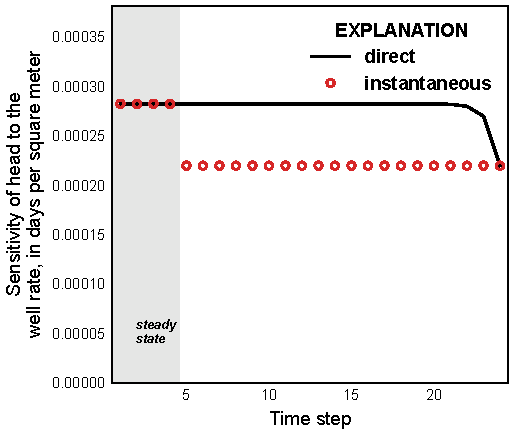
\includegraphics{Figures/instantaneous.pdf}
	\caption{Sensitivity of head at an observation cell to the rate of a well, computed as a direct measure and as an instantaneous measure, for a model whose first stress period is steady state (shaded) and whose remaining periods are transient. Both forms carry an observation at every time step. The two agree at the four steady-state steps and at the last step solved, and differ at the transient steps between them.}
	\label{fig:instantaneous}
\end{figure}

\section*{What it is for}

The map of equation~\ref{eqn:inst-kernel} answers a question about the present: where does a stress applied now have the most effect on the measured quantity now. Held against a stream or a lake, it locates the cells whose pumping is felt immediately by that boundary, which is the quantity a short-horizon management problem is written in terms of. It is also inexpensive, because only the observed steps are solved: a measure observed at one time in a two hundred step simulation costs one solve rather than two hundred.

The independence of the observed steps is the other reason to prefer it. Every entry of an instantaneous measure reports the same map it would report alone, so the entries of one measure can be read as separate answers. The entries of a direct measure cannot, because each carries the influence of those after it.

\section*{What it is not for}

An instantaneous measure does not give the response of the measured quantity to a stress applied at an earlier time. That response is what makes drawdown deepen while a well runs, and it is carried by exactly the passing between time steps that this form drops. Adding the maps of successive steps together does not recover it, because each map reports the effect of a stress applied within its own step and none of them reports the effect that stress continues to have afterward.

The consequence is worth stating plainly, because the sum is a natural thing to try. Accumulated over a simulation in which a well pumps at a constant rate, the maps grow the drawdown linearly with the number of steps, while the drawdown of a confined aquifer grows with the logarithm of time. The accumulation is therefore exact after the first time step, where there is no earlier stress to account for, and departs from the simulated drawdown thereafter.

A measure whose answer depends on the history of the stresses, including drawdown through time and the response matrix that reconstructs it, needs the direct form.


\chapter{Formulation and Exactness}
\label{ch:formulation}
The adjoint solution is taken from the matrix \mf{} assembled while it solved the flow model. Whether that matrix is the derivative of the flow equations, or only the operator used to iterate toward their solution, depends on the formulation the flow model was run under. This chapter describes when a sensitivity is exact, when it is a partial derivative, and what \adj{} reports.

\section*{Two matrices}

A cell that converts between confined and unconfined carries a transmissivity that follows the head, because the saturated thickness does. Writing the flow between cells $n$ and $m$ as

\begin{equation}
	\label{eqn:formulation-flow}
	Q_{nm} = C_{nm}(h)\left( h_{m} - h_{n} \right),
\end{equation}

\noindent where $C_{nm}$ is the conductance between the two cells (L$^{2}$T$^{-1}$), the derivative of the residual with respect to the head carries two terms,

\begin{equation}
	\label{eqn:formulation-jacobian}
	\frac{\partial r_{n}}{\partial h_{n}} = -\sum_{m} C_{nm}
	+ \sum_{m} \frac{\partial C_{nm}}{\partial h_{n}}
	\left( h_{m} - h_{n} \right).
\end{equation}

Under the Newton-Raphson formulation \mf{} assembles both terms of equation~\ref{eqn:formulation-jacobian}, because that is what the method requires. Under the standard formulation it assembles only the first and lags the second, recomputing the conductance between iterations until the heads stop moving. Both converge to a solution of the same physical problem, but only the first leaves behind a matrix that is the derivative of the equations.

The adjoint needs that derivative. Given the first term alone it returns a partial derivative, holding the transmissivity fixed in the same way that holding a lake stage fixed returns a partial derivative (Chapter~\ref{ch:lake}).

\section*{How far it is out}

A single-layer unconfined model was pumped by a well against a general-head boundary, and the sensitivity of a head to the well rate compared with a central difference. The model was run twice at each rate, once under each formulation.

\begin{table}[htb]
	\centering
	\caption{Error in the sensitivity of a head to a well rate, against a
	finite-difference derivative, under each formulation.}
	\label{tab:formulation}
	\small
	\begin{tabular}{lrr}
		\toprule
		\shortstack[l]{Head in the\\pumped cell} &
		\shortstack[r]{Newton-\\Raphson} &
		\shortstack[r]{Standard\\formulation} \\
		\midrule
		5.46 & 0.000\% & 5.9\%   \\
		2.20 & 0.000\% & 10.2\%  \\
		\bottomrule
	\end{tabular}
\end{table}

The error under the standard formulation grows as the cell empties, which is what the neglected term in equation~\ref{eqn:formulation-jacobian} would give: the conductance follows the head most steeply where the saturated thickness is least. A confined model is unaffected, because there the conductance does not follow the head at all and the two matrices are the same.

A second head-dependent term compounds this. A well given \texttt{AUTO\_FLOW\_REDUCE} has its rate scaled by a smooth function of the head in its cell, and that dependence is likewise carried into the matrix only under the Newton-Raphson formulation. On the same model the sensitivity was in error by 146 percent with the reduction active and the standard formulation in use, against 10 percent for the same model with no reduction at all. Under the Newton-Raphson formulation the reduced well is exact, matching a central difference to six figures, where neglecting the reduction entirely would be out by a factor of nearly five.

\section*{What is reported}

\adj{} reports a flow model that has convertible cells and was not run under the Newton-Raphson formulation, and reports a reduced well separately, rather than returning either as though it were exact. Neither is reported for a model run under Newton-Raphson, where both are carried.

\section*{Limitation}

The neglected term is not recovered. It cannot be taken from the Newton-Raphson assembly, because the two formulations do not solve the same discrete equations: the Newton-Raphson formulation weights the conductance upstream, and the converged heads of the two runs differ. Recovering it means differentiating the conductance the standard formulation actually used, which is one of three cell-averaging schemes, over horizontal, vertical, and vertically staggered connections. Running the flow model under the Newton-Raphson formulation is the shorter path to an exact sensitivity, and is what \adj{} recommends where it reports the condition.


\chapter{Storage}
\label{ch:storage}
Storage is the only term in the groundwater flow equations that connects one time step to the next, so it is the term through which an adjoint solution propagates backward in time. This chapter describes that coupling and the selection between the specific-storage and specific-yield contributions.

\section*{Coupling between time steps}

The right-hand side at time step $k$ depends on the head at step $k-1$ through the storage terms. Differentiating the adjoint problem with respect to that earlier head gives the term that carries the later adjoint state backward, which is what an instantaneous measure drops (Chapter~\ref{ch:instantaneous}). Writing it per cell,

\begin{equation}
	\label{eqn:drhsdh}
	\frac{\partial b}{\partial h^{k-1}} = -\left(
	\frac{\partial Q_{SS}}{\partial h^{k-1}} +
	\frac{\partial Q_{SY}}{\partial h^{k-1}} \right),
\end{equation}

\noindent where $Q_{SS}$ and $Q_{SY}$ are the volumetric flow rates from specific storage and specific yield (L$^{3}$T$^{-1}$).

The quantity in equation~\ref{eqn:drhsdh} is formed while the forward model runs and stored with that time step. It is paired with the adjoint state of the \emph{following} step, so the saturation it requires is the one at the step where it is formed, which the following step sees as the previous saturation.

\section*{Selecting the contributions}

\mf{} does not apply both contributions at once. The selection is made on the saturation of the cell at the previous time step, and it depends on the options in effect \citep{langevin2017}.

\subsection*{Specific yield}

Specific yield enters the previous-head derivative only through the saturation. For a cell that is neither full nor dry, $S_F^{k-1} = (h^{k-1} - BOT)/\Delta z$ and so $\partial S_F^{k-1} / \partial h^{k-1} = 1/\Delta z$, giving

\begin{equation}
	\label{eqn:dsy}
	\frac{\partial Q_{SY}}{\partial h^{k-1}} = \frac{S_y A}{\Delta t^{k}},
\end{equation}

\noindent where $S_y$ is the specific yield (dimensionless), $A$ is the horizontal area of the cell (L$^{2}$), and $\Delta t^{k}$ is the length of the time step (T). Once the cell is full or dry the saturation stops changing with head, the derivative in equation~\ref{eqn:dsy} vanishes, and specific yield drops out.

\subsection*{Specific storage}

The specific-storage contribution depends on which formulation is active. Under the default formulation the previous-head derivative follows the previous saturation,

\begin{equation}
	\label{eqn:dss-default}
	\frac{\partial Q_{SS}}{\partial h^{k-1}} =
	\frac{SC1}{\Delta t^{k}} S_F^{k-1}, \qquad SC1 = S_s A \Delta z,
\end{equation}

\noindent where $S_s$ is the specific storage coefficient (L$^{-1}$), $SC1$ is the primary storage coefficient (L$^{2}$), and $\Delta z$ is the cell thickness (L). Under the \texttt{SS\_CONFINED\_ONLY} option, specific storage acts only where the cell is full, and the term is removed rather than scaled:

\begin{equation}
	\label{eqn:dss-confined}
	\frac{\partial Q_{SS}}{\partial h^{k-1}} = \begin{cases}
		\dfrac{SC1}{\Delta t^{k}}, & S_F^{k-1} = 1, \\[2ex]
		0, & S_F^{k-1} < 1.
	\end{cases}
\end{equation}

A cell that is not convertible is treated as full at all times, and equation~\ref{eqn:dss-default} reduces to $SC1/\Delta t^{k}$.

Equations~\ref{eqn:dsy} through \ref{eqn:dss-confined} are complementary on the same test. Specific storage acts where the cell was full, specific yield where it was not.

\section*{Sensitivity to the storage parameters}

The terms above carry the adjoint solution backward through time. Specific storage and specific yield are also parameters of the flow model in their own right, and a performance measure has a sensitivity to each. They are reported separately, because they describe different water: specific storage the water an aquifer yields by compressing while it stays full, specific yield the water it drains from the pore space as the water table falls. A model calibrated against one is not thereby calibrated against the other.

Both follow from the same flows. Differentiating the specific-storage flow of equation~\ref{eqn:drhsdh} with respect to $S_s$ gives

\begin{equation}
	\label{eqn:dqdss}
	\begin{split}
	\frac{\partial Q_{SS}}{\partial S_s} = \frac{A \Delta z}{\Delta t^{k}}
	\Big[ & S_F^{k-1} h^{k-1} - S_F^{k} h^{k} \\
	& + BOT \left( S_F^{k} - S_F^{k-1} \right) \\
	& + \frac{\Delta z}{2} \left( \left(S_F^{k}\right)^{2}
	- \left(S_F^{k-1}\right)^{2} \right) \Big],
	\end{split}
\end{equation}

\noindent and the specific-yield flow, which is the water held between the saturations at the two ends of the step, gives

\begin{equation}
	\label{eqn:dqdsy}
	\frac{\partial Q_{SY}}{\partial S_y} = \frac{A \Delta z}{\Delta t^{k}}
	\left( S_F^{k-1} - S_F^{k} \right).
\end{equation}

Both expressions need the saturation at each end of the step. Equation~\ref{eqn:dqdsy} is nothing but the difference between them, so a saturation taken twice from the same end reduces it to zero, and equation~\ref{eqn:dqdss} to the term in the heads alone.

Under \texttt{SS\_CONFINED\_ONLY} the saturation is one at or above the top of the cell and zero below it, and specific storage acts only where the cell is full, so equation~\ref{eqn:dqdss} reduces to

\begin{equation}
	\label{eqn:dqdss-confined}
	\begin{split}
	\frac{\partial Q_{SS}}{\partial S_s} = \frac{A \Delta z}{\Delta t^{k}}
	\Big[ & \left. \left( TOP - h^{k} \right) \right|_{S_F^{k} = 1} \\
	& + \left. \left( h^{k-1} - TOP \right) \right|_{S_F^{k-1} = 1} \Big].
	\end{split}
\end{equation}

The two halves are taken on the saturation at their own end of the step, so a cell that is full at the start and not at the end carries the first half and not the second.

\section*{Verification}

A seven by seven single-layer model was drawn down by a well over four time steps, leaving the cells between about half and four-fifths saturated. The sensitivity of the head at an observation cell to the pumping rate was compared with a finite-difference derivative taken by perturbing that rate.

\begin{table}[htb]
	\centering
	\caption{Error in the head sensitivity against a finite-difference
	derivative, before and after the contributions were selected as described
	in this chapter.}
	\label{tab:sto-verify}
	\small
	\begin{tabular}{lrr}
		\toprule
		Formulation &
		\shortstack[r]{Applying $SC1$\\throughout} &
		\shortstack[r]{Selecting on\\saturation} \\
		\midrule
		\texttt{SS\_CONFINED\_ONLY} & 10.7\% & 0.17\% \\
		Default                     & 2.6\%  & 0.15\% \\
		\bottomrule
	\end{tabular}
\end{table}

Applying $SC1$ at full cell thickness everywhere gives a partially saturated cell a storage term the forward model does not have, and Table~\ref{tab:sto-verify} shows the resulting error. The residual error after the correction is consistent with the nonlinearity of the finite-difference derivative itself.

The sensitivities to the storage parameters themselves were checked on the same model, against finite-difference derivatives taken by perturbing each parameter in turn.

\begin{table}[htb]
	\centering
	\caption{Sensitivity to each storage parameter as a fraction of a
	finite-difference derivative in that parameter, before and after the
	derivatives were taken over the saturations at both ends of the time step.}
	\label{tab:sto-parameters}
	\small
	\begin{tabular}{lrr}
		\toprule
		Parameter &
		\shortstack[r]{Saturation\\taken once} &
		\shortstack[r]{Saturation at\\both ends} \\
		\midrule
		Specific storage & 0.9844       & 1.0000 \\
		Specific yield   & not reported & 1.0010 \\
		\bottomrule
	\end{tabular}
\end{table}

Equation~\ref{eqn:dqdsy} is the difference between the saturations at the two ends of the step, so taking both from the same end leaves it identically zero and there is no specific-yield sensitivity to report. The saturation the first time step starts from is the one the initial heads imply, and reading it before the flow model has formed it, when the array still holds the value it was allocated with, is enough on its own to change the sign of the summed specific-storage sensitivity.

The error is largest under \texttt{SS\_CONFINED\_ONLY} because that option removes the term entirely rather than reducing it, so the difference between applying and not applying it is the whole term. The size of the error in a given model scales with $S_s \Delta z$ relative to $S_y$: where a model sets $S_s$ such that $S_s \Delta z$ is comparable to or larger than $S_y$, an unselected specific-storage term dominates the coupling between time steps.

\section*{Limitation}

The \texttt{ORIGINAL\_SPECIFIC\_STORAGE} option, which restores the formulation used before \mf{} version 6.1.3, is not supported. Its previous-head derivative carries a term in the previous head itself in addition to the saturation, and \adj{} reports the option as unsupported rather than approximating it.


\chapter{Lake Package}
\label{ch:lake}
A lake stage is a dependent variable of the simulation, but by default the Lake (LAK) Package does not add its equations to the groundwater flow matrix: the stage is solved in the outer iteration. An adjoint solution built from the flow matrix alone therefore treats the stage as fixed, and reports only the part of a sensitivity that travels through the aquifer. This chapter describes how the lake water balance is brought into the adjoint system.

\section*{The fixed-stage error}

Consider pumping near a lake. The heads beneath the lake fall, which increases the leakage from the lake to the aquifer; the lake stage then falls too, which reduces the leakage that the lower heads would otherwise have drawn. A sensitivity computed with the stage held fixed captures the first effect and not the second, so it does not answer the question a capture analysis asks \citep[for example,][]{leake2010,barlow2012}.

The stage cannot simply be added to the flow matrix, because \mf{} does not put it there. Instead the adjoint system is extended.

\section*{Bordered system}

Let $\mathbf{h}$ be the cell heads and $\mathbf{s}$ the stages of the lakes whose stage is free to move. Write the aquifer residual as $\mathbf{r}$, as in equation~\ref{eqn:residual}, and the lake water balance as $\mathbf{r}_{L}$. The two sets of equations together are

\begin{equation}
	\label{eqn:lak-bordered}
	\begin{bmatrix}
		\dfrac{\partial \mathbf{r}}{\partial \mathbf{h}} &
		\dfrac{\partial \mathbf{r}}{\partial \mathbf{s}} \\[2ex]
		\dfrac{\partial \mathbf{r}_{L}}{\partial \mathbf{h}} &
		\dfrac{\partial \mathbf{r}_{L}}{\partial \mathbf{s}}
	\end{bmatrix}
	\begin{bmatrix} \mathbf{h} \\ \mathbf{s} \end{bmatrix}
	=
	\begin{bmatrix} \mathbf{b} \\ \mathbf{b}_{L} \end{bmatrix}.
\end{equation}

The leading block is the matrix $\left[ \mathbf{A} \right]^{k}$ of equation~\ref{eqn:forward}. The other three blocks add one row and one column per free lake, which is why this is called a bordered matrix: the original system sits inside a border one equation deep. The adjoint problem is the transpose of equation~\ref{eqn:lak-bordered}, and its solution has one extra entry per lake alongside the usual one per cell.

A lake with a specified stage contributes no unknown and is left out of the border, as is an inactive lake.

\subsection*{Connection terms}

Each lake-aquifer connection carries a conductance $C_{n,\ell}$ (L$^{2}$T$^{-1}$) between cell $n$ and lake $\ell$. The exchange depends on both the head in the cell and the stage of the lake, giving the off-diagonal blocks

\begin{equation}
	\label{eqn:lak-offdiag}
	\frac{\partial r_{n}}{\partial s_{\ell}} = C_{n,\ell}, \qquad
	\frac{\partial r_{L,\ell}}{\partial h_{n}} = \mathrm{HCOF}_{n},
\end{equation}

\noindent summed over the connections between cell $n$ and lake $\ell$, and the conductance also accumulates on the lake's own diagonal.

The two halves of equation~\ref{eqn:lak-offdiag} are not written the same way, and the difference matters. A lake perched above the water table leaks at a rate set by its bed rather than by the head beneath it. \mf{} marks that state by leaving \texttt{HCOF} at zero for the connection while the exchange still follows the stage. Using the conductance on both sides gives a lake perched above a falling water table a head sensitivity it does not have; using \texttt{HCOF} on the head side and the conductance on the stage side reproduces the two cases with one expression.

\subsection*{Storage and surface area}

A transient step adds the change in lake storage to the diagonal, $\partial V / \partial s$ divided by the time step length, where $V$ is the lake volume (L$^{3}$) and $s$ is the lake stage (L). A steady-state step adds nothing.

A lake whose surface area grows with stage evaporates more as it rises and catches more rain, and those act in opposite senses, so the diagonal also carries

\begin{equation}
	\label{eqn:lak-surface}
	\left( E - P \right) \frac{\partial S_{A}}{\partial s},
\end{equation}

\noindent where $E$ is the evaporation rate (LT$^{-1}$), $P$ the rainfall rate (LT$^{-1}$), and $S_{A}$ the lake surface area (L$^{2}$). Where the lake geometry is given as a table of stage against volume and area, the derivatives $\partial V / \partial s$ and $\partial S_A / \partial s$ are the slopes of the interval of the table holding the current stage, matching the interpolation \mf{} performs.

As with the aquifer, the lake storage term also couples one time step to the next, and the stage part of the adjoint solution is carried backward in the same way. An instantaneous measure, for which the time steps are independent, does not carry it (Chapter~\ref{ch:instantaneous}).

\subsection*{Outlets}

An outlet discharges over an invert according to its type: a specified rate, a Manning rating, or a weir. Each is a power of the depth $d$ over the invert, so the derivative follows from the discharge itself,

\begin{equation}
	\label{eqn:lak-outlet}
	\frac{\partial Q_{\mathrm{out}}}{\partial s} = \gamma
	\frac{Q_{\mathrm{out}}}{d}, \qquad
	\gamma = \begin{cases}
		0, & \text{specified rate}, \\
		5/3, & \text{Manning}, \\
		3/2, & \text{weir}.
	\end{cases}
\end{equation}

Writing the derivative in terms of the reported discharge rather than recomputing the rating avoids reproducing the roughness, width, and slope of the outlet. Where an outlet discharges from one lake into another, the derivative also appears off the diagonal, coupling the two lake rows.

Very close to the invert \mf{} smooths the rating to zero. That smoothing is not reproduced here, so an outlet with a depth below $10^{-6}$ in model length units is treated as carrying no flow.

\section*{Verification}

\begin{figure}[htb]
	\centering
	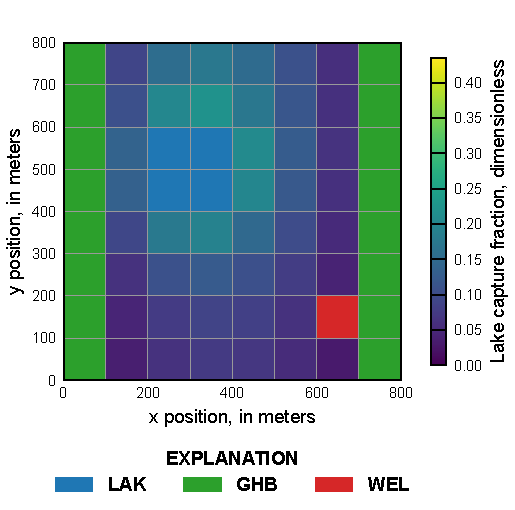
\includegraphics{Figures/lake-capture.pdf}
	\caption{Lake capture fraction for the model the lake tests use, the
	fraction of a withdrawal at a cell that is drawn from the lake rather than
	from storage or from another boundary, for the second model layer, in which
	it is largest. LAK marks the cells the lake connects to, GHB the
	general-head boundaries that hold the heads at the left and right edges of
	the model, and WEL the pumped cell. The lake is incised into the top layer,
	which is inactive beneath it, and reaches the aquifer through one vertical
	connection per cell into the layer shown, so the capture is the response the
	water balance of this chapter describes, without the approximations noted at
	the end.}
	\label{fig:lake-capture}
\end{figure}

A lake sitting in a two layer model was pumped from a cell away from it, and the resulting change in lake exchange compared with the difference between two forward runs. The adjoint reports a capture of $-3.4232 \times 10^{-2}$ against a two-run difference of $-3.4258 \times 10^{-2}$, a difference of 0.08 percent. The model is the one the lake tests use, so the figure shows the lake whose behavior those tests check. Capture fractions across that model are shown in figure~\ref{fig:lake-capture}. With the stage held fixed the adjoint reported a lake capture of $-4.1 \times 10^{-3}$ against a two-run difference of $-4.6 \times 10^{-3}$, an error of about a factor of two in the part of the response the stage carries. Solving the water balance with the flow equations reduced the discrepancy to $-5 \times 10^{-4}$.

The residual discrepancy is not numerical. It is accounted for by two couplings that remain outside the border: inflow routed to the lake by the Water Mover (MVR) Package, which follows the state of the package supplying it, and the dependence of a horizontal connection's conductance on the saturated fraction of the cell it connects to.


\chapter{Streamflow Routing Package}
\label{ch:sfr}
A reach depth follows the flow through the reach, so like a lake stage it is a dependent variable that the Streamflow Routing (SFR) Package solves outside the groundwater flow matrix. The adjoint system is bordered in the same way as for a lake, described in Chapter~\ref{ch:lake}, with one equation per reach. What distinguishes the stream case is that those equations are not independent of one another: they carry the routing of water from reach to reach.

\section*{Reach equation}

\mf{} sets the depth $d$ of a reach so that the Manning discharge equals the mean of the flow entering and leaving it,

\begin{equation}
	\label{eqn:sfr-balance}
	q_{\mathrm{man}}(d) = \tfrac{1}{2}\left( Q_{\mathrm{in}} +
	Q_{\mathrm{out}} \right), \qquad
	Q_{\mathrm{out}} = Q_{\mathrm{in}} - Q_{\mathrm{leak}},
\end{equation}

\noindent where $Q_{\mathrm{leak}}$ is the exchange with the aquifer (L$^{3}$T$^{-1}$) and $d$ is the reach depth (L). For a reach without a cross section the wetted perimeter is the reach width, which carries no dependence on depth, so the discharge is a power of the depth,

\begin{equation}
	\label{eqn:sfr-manning}
	q_{\mathrm{man}}(d) = \frac{K w \sqrt{S}}{n}\, d^{5/3},
\end{equation}

\noindent with $w$ the width (L), $S$ the slope (dimensionless), $n$ Manning's roughness, and $K$ a unit conversion. The derivative needed for the border follows directly,

\begin{equation}
	\label{eqn:sfr-dqdd}
	\frac{\partial q_{\mathrm{man}}}{\partial d} = \frac{5}{3}
	\frac{q_{\mathrm{man}}}{d}.
\end{equation}

Equation~\ref{eqn:sfr-dqdd} is written in terms of the discharge \mf{} reports rather than rebuilding the rating from $K$, $w$, $S$, and $n$. The unit conversion in particular varies with the model's unit system, and taking the reported discharge makes the derivative correct without reproducing it.

Below a depth of $10^{-5}$ in model length units \mf{} smooths the discharge to zero. That smoothing is not reproduced, so a shallower reach is treated as carrying no flow.

\section*{Reaches with a cross section}

A reach may instead be given a cross section, a set of points describing the shape of the channel as a station across it and a height above the streambed. The channel is then a chain of straight segments between those points, and the discharge is the conveyance of the wetted part of each,

\begin{equation}
	\label{eqn:sfr-section}
	q_{\mathrm{man}}(d) = K \sqrt{S} \sum_{i} \frac{a_{i}^{5/3}}
	{n_{i} \, p_{i}^{2/3}},
\end{equation}

\noindent where $a_{i}$ is the wetted area of segment $i$ (L$^{2}$), $p_{i}$ is its wetted perimeter (L), and $n_{i}$ is Manning's roughness of the reach times the roughness fraction given for that segment. Equation~\ref{eqn:sfr-manning} is the special case of a single segment whose perimeter does not follow the depth, and equation~\ref{eqn:sfr-dqdd} does not hold for equation~\ref{eqn:sfr-section}.

Both the area and the perimeter of a segment follow the depth, so the derivative is taken from them rather than from a perturbation of the discharge,

\begin{equation}
	\label{eqn:sfr-dsection}
	\frac{\partial q_{\mathrm{man}}}{\partial d} = K \sqrt{S} \sum_{i}
	\frac{1}{n_{i}} \left(
	\frac{5}{3} \frac{a_{i}^{2/3}}{p_{i}^{2/3}}
	\frac{\partial a_{i}}{\partial d} -
	\frac{2}{3} \frac{a_{i}^{5/3}}{p_{i}^{5/3}}
	\frac{\partial p_{i}}{\partial d} \right).
\end{equation}

The area of a segment grows with the depth at its wetted top width, and its perimeter grows at the length of the wetted face, so both derivatives in equation~\ref{eqn:sfr-dsection} come from the geometry of the section and neither needs the discharge. Both step where the water surface passes a point of the section, and the derivative is taken on the side the depth is on.

A cross section carries a second consequence. The streambed conductance of a reach is proportional to its wetted perimeter, and for a section that perimeter follows the depth, so the leakage responds to the depth through the conductance as well as through the stage,

\begin{equation}
	\label{eqn:sfr-dleak}
	\frac{\partial Q_{\mathrm{leak}}}{\partial d} = C \left(
	1 + \frac{1}{P} \frac{\partial P}{\partial d}
	\left( h_{s} - h \right) \right),
\end{equation}

\noindent where $C$ is the streambed conductance (L$^{2}$T$^{-1}$), $P$ is the wetted perimeter of the whole section (L), $h_{s}$ is the reach stage (L), and $h$ is the head beneath the reach (L), taken at the bottom of the streambed where the reach is perched. A reach without a cross section has a perimeter that does not follow the depth, the bracket in equation~\ref{eqn:sfr-dleak} is one, and the leakage derivative is the conductance alone. Only the bracket is formed from the section, so the conductance the package reports sets the magnitude and a reach on an inactive cell stays at zero.

\section*{Routing}

The flow entering a reach is the sum of the flows leaving the reaches upstream of it, apportioned by the diversion fractions specified for the network. The connectivity is that of the stream network itself, which identifies the reaches upstream of each reach.

Because $Q_{\mathrm{out}}$ of an upstream reach depends on that reach's depth and on its leakage, differentiating equation~\ref{eqn:sfr-balance} produces entries away from the diagonal in two places. The first couples one reach row to another,

\begin{equation}
	\label{eqn:sfr-updepth}
	\frac{\partial}{\partial d_{u}} \; \tfrac{1}{2} Q_{\mathrm{in}} =
	\tfrac{1}{2}\, \sigma \, \frac{\partial q_{\mathrm{man},u}}
	{\partial d_{u}},
\end{equation}

\noindent where $\sigma$ is the fraction of the upstream reach's outflow routed to this one (dimensionless). The second reaches back into the aquifer, because the flow leaving the upstream reach carries half of that reach's leakage,

\begin{equation}
	\label{eqn:sfr-uphead}
	\frac{\partial}{\partial h_{u}} \; \tfrac{1}{2} Q_{\mathrm{in}} =
	\tfrac{1}{2}\, \sigma \, \mathrm{HCOF}_{u}.
\end{equation}

The sign of equation~\ref{eqn:sfr-uphead} is easy to get wrong, and an error there is not obvious in the result: it produces sensitivities of a plausible magnitude that are wrong by a modest factor. Checking the assembled block against a finite-difference Jacobian is what identified it.

\section*{Flow-limited reaches}

A reach can be asked to lose more water than it carries. \mf{} limits the leakage to the available flow, and marks that state by leaving both the reach's \texttt{HCOF} and the change in its outflow at zero: the reach passes on nothing and its leakage no longer responds to the head beneath it.

The derivative structure changes accordingly. The reach's own depth no longer sets its leakage, so the coupling moves to the reaches upstream that supply it, and a correction appears that connects one aquifer cell directly to another, bypassing the reach equation. That correction is folded into the aquifer block of the bordered matrix rather than the border itself.

\section*{Verification}

\begin{figure}[htb]
	\centering
	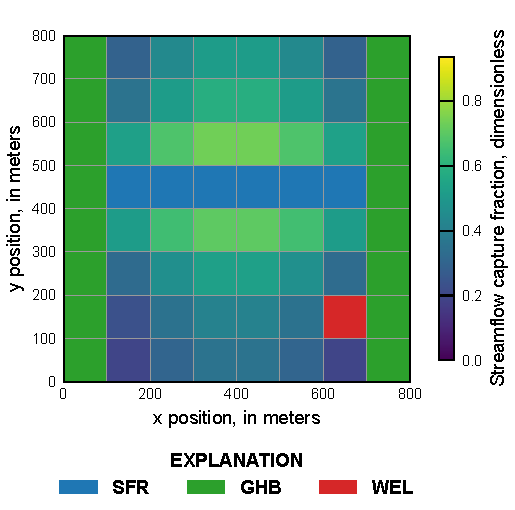
\includegraphics{Figures/sfr-capture.pdf}
	\caption{Streamflow capture fraction for the model the streamflow tests
	use, the fraction of a withdrawal at a cell that is drawn from the stream
	rather than from storage or from another boundary. SFR marks the cells the
	reaches occupy, GHB the general-head boundaries that hold the heads at the
	left and right edges of the model, and WEL the pumped cell. The reach depths
	are solved with the flow equations as described in this chapter.}
	\label{fig:sfr-capture}
\end{figure}

A chain of reaches crossing a single layer model was pumped from a cell away from the stream, and the resulting change in reach exchange compared with the difference between two forward runs. The adjoint reports a capture of $-2.32472 \times 10^{-1}$ against a two-run difference of $-2.32470 \times 10^{-1}$. Capture fractions across that model are shown in figure~\ref{fig:sfr-capture}. On a valley model routing a longer network, holding the reach depths fixed gave a discrepancy of about 26 percent, and solving the reach equations with the flow equations reduced it to 0.04 percent.

A branching network, in which one reach receives water from two upstream reaches and the apportionment fractions therefore matter, reproduces its finite-difference sensitivities to the same tolerance.

A diversion was added to the same model and run under each of the four rules. Holding the diverted flow fixed gave sensitivities in error by 0.03 to 0.11 percent under the three rules whose derivative is not zero, and carrying equations~\ref{eqn:sfr-passed} and \ref{eqn:sfr-diverted} brought all four to within 0.001 percent. Under \texttt{THRESHOLD} the derivative is zero, and holding the flow fixed was already exact.

The same model was run again with a trapezoidal cross section on every reach. The rating of equation~\ref{eqn:sfr-section} reproduces the discharge the forward model solved each depth against to eleven significant figures, which is the check that established the geometry before any derivative was taken from it, and the derivative of equation~\ref{eqn:sfr-dsection} matches a central difference of that rating to nine, on both sides of a break in the section. Holding the depths of those reaches fixed gave a capture sensitivity in error by 1.7 percent, and carrying equations~\ref{eqn:sfr-dsection} and \ref{eqn:sfr-dleak} reduced it to 0.002 percent.

\section*{Diversions}

A diversion takes water out of the flow a reach passes on, under one of four rules. Writing $v$ for the rate the diversion is given (L$^{3}$T$^{-1}$, or dimensionless for a fraction) and $q$ for the flow available to it when its turn comes (L$^{3}$T$^{-1}$), the rules and the derivative each carries are given in Table~\ref{tab:sfr-rules}.

\begin{table}[htb]
	\centering
	\caption{The four diversion rules, the flow each takes, and how that flow
	follows the flow available to the diversion.}
	\label{tab:sfr-rules}
	\small
	\begin{tabular}{lll}
		\toprule
		Rule & Diverted & $\partial / \partial q$ \\
		\midrule
		\texttt{FRACTION}  & $q v$          & $v$ \\
		\texttt{EXCESS}    & $\max(q - v, 0)$ & 1 above $v$ \\
		\texttt{UPTO}      & $\min(v, q)$     & 1 below $v$ \\
		\texttt{THRESHOLD} & $v$ if $q \geq v$ & 0 \\
		\bottomrule
	\end{tabular}
\end{table}

Three of the four are piecewise, so the derivative steps where the rule switches, in the same way that the derivative of a lake connection steps as the connection becomes perched. That is workable away from the switch.

Which rule is in effect cannot be read from the simulation, because \mf{} keeps it as text rather than among the quantities it exposes. It does not have to be. The flow available to a diversion, the rate it was given, and the flow it took are all recoverable, and those three determine the derivative. Where two rules give the same diverted flow they also give the same derivative: \texttt{THRESHOLD} and \texttt{UPTO} both hold at the rate once the flow exceeds it, and \texttt{THRESHOLD} and \texttt{EXCESS} both take nothing below it. The rule itself can therefore stay unknown.

The diversions of a reach are applied in turn, each taking from what the one before it left, so writing $g_{i}$ for the derivative of diversion $i$ the flow passed on to the reaches below carries

\begin{equation}
	\label{eqn:sfr-passed}
	\frac{\partial q_{\mathrm{out}}}{\partial q} = \prod_{i} \left( 1 - g_{i} \right),
\end{equation}

\noindent and the reach a diversion feeds receives

\begin{equation}
	\label{eqn:sfr-diverted}
	\frac{\partial q_{i}}{\partial q} = g_{i} \prod_{j < i} \left( 1 - g_{j} \right).
\end{equation}

Equations~\ref{eqn:sfr-passed} and \ref{eqn:sfr-diverted} scale the routing coefficient of equation~\ref{eqn:sfr-updepth} rather than adding structure of their own, so a diversion enters the bordered system only through the share one reach sends another. The share itself is taken from the total \mf{} keeps for each reach, which leaves out both a diversion and an inactive reach, rather than summed from the fractions given to the reaches below, which would count a diversion in the denominator.

\section*{Limitations}

The flows leave the rule open only where two rules divert the same amount and respond differently, which takes a coincidence between the flow available and the rate the diversion is given. A flow of exactly twice the rate is one: \texttt{EXCESS} passes the rate on and takes the rest, which is then the rate itself, the same amount \texttt{UPTO} and \texttt{THRESHOLD} take, and the three do not agree on how that amount would change. Where that happens \adj{} reports the diversion and holds its flow fixed rather than returning a partial derivative silently.

A reach whose outflow is not positive diverts nothing under any rule, and passes nothing on, so no rule is inferred for it and none is needed.



\bibliography{references}

\end{document}
